\section{ICN IoT Middleware System Design}
In this section, we will propose a overall system design formed by three distributed physical components(shown in Figure~\ref{fig:phy})--Aggregator, Local Service Gateway, and IoT server. They cover four principle functionality to develop IoT middleware over ICN network. In legacy IP-based IoT platform, these functionality are almost implemented on a centralized server, or over-lay application. In our ICN-IoT middleware architecture, they are pushed down to distributed components which can form a self-configuring subsystem to provide local service as well as a complete system that enables global communication. 
\begin{figure}
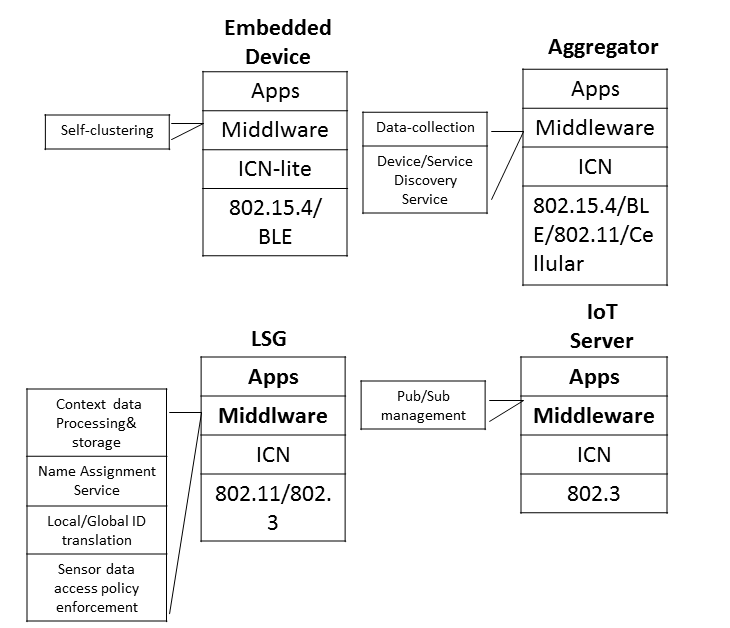
\includegraphics[width=\columnwidth]{figure/physical_comp.png}
\caption{\label{fig:phy}Physical components of ICN-IoT middleware}
\end{figure}
\subsection{Physical Components}\label{sec:physical}
\begin{itemize}
\vspace{-2pt}\item{\em Aggregator}:
is the base-line component in our middlware architecture that interconnects the various IoT service in the local network. A Aggregator usually acts as gateway for resource-constraint wireless sensors, or it can be a device that integrates sensing/actuating service. 
\vspace{-2pt}\item{\em Local Service Gateway (LSG)}:
connects the local IoT system to the outside world. It handles local name assignment and sensor data access policy enforcement. Furthermore, context data processing service can be implemented within this entity to publish only the information abstraction to IoT server.    
\vspace{-2pt}\item{\em IoT Server}:
is a centralized server that maintains subscription membership and provides lookup service for the subscriber. Legacy IoT server also involves in the data path from publisher to subscriber, where the bandwidth of its interfaces could be a bottleneck. In contrast, IoT server in our architecture only involves in control path in which publisher and subscriber exchange their names and certificates.  
\end{itemize}

We will discuss the breakdown functionality of each  physical component in following subsection to demonstrate detail protocol design.
\subsection{Device Discovery}
The objective of device discovery is to contextually establish relationship for nodes in proximity and remote. Device discovery is a key component of any IoT system, which can be considerably simplified by the ICN network. In today's IoT systems, the IP overlay device discovery module not only focuses on the reach-ability of a device, but also the device physical properties\cite{iotivity,alljoyn}. However, a translation service is required to maintain the mapping from network addresses to physical attributes and manual configuration is necessary. In contrast, ICN uses names to discover new devices, without involving manual configuration or name translation. Below, we explain the ICN-IoT device discovery process in detail, including both devices that are able to run  full-stack protocols (referred to as \emph{resource-rich sensors}) and devices that are unable to do so (referred to as \emph{resource-constrained sensors}).

\vspace{1mm}\noindent{\bf Resource-rich sensors}: Many resource-rich sensors come with manufacture secure ID and model name, which need to be exposed to the aggregator and LSG to facilitate device discovery. This objective is achieved in different ways by NDN and MF.  In NDN, this process is initiated by the configuration service running on LSG, which periodically broadcasts discovery Interests (using the name $/iot/model$). The new sensor replies to the discovery interest with its information, and the configuration service then registers the sensor and generates a local ICN name for the sensor. In MF, we can set the model number, $group-GUID$, as the destination address, and configuration service issues the request via multicasting. On receiving of the request, the new device replies with the manufacture secure ID, and the configuration service register and generates a local ICN name for the new device.


\vspace{1mm}\noindent{\bf Resource-constrained sensors}: Many resource-constrained sensors connect to the Internet using the IEEE 802.15.4 technology via a border router~\cite{hui2008ip}. These sensors voluntarily discover each other in proximity and establish forwarding paths to the border router, self-organizing into a mesh network. Similarly, Aggregator in our ICN-IoT middleware acts as a border router, and neighbor discovery among sensors is achieved differently in NDN and MF. In NDN, when a new sensor arrives, it broadcasts a neighbor discovery message to connect with neighbors. After establishing connectivity with neighboring sensors, it broadcasts an Interest named $/ndn/aggregatorservice$ to discover the Aggregator. In MF, neighbor discovery is naturally supported, and the new sensor simply needs to send a discovery request to a well-known broadcast GUID to discover the Aggregator. %On receiving, the target Aggregator receives the request and registers the new device if there is matched service name.
The above process is shown as Figure~\ref{fig:device_dis}.
\begin{figure}
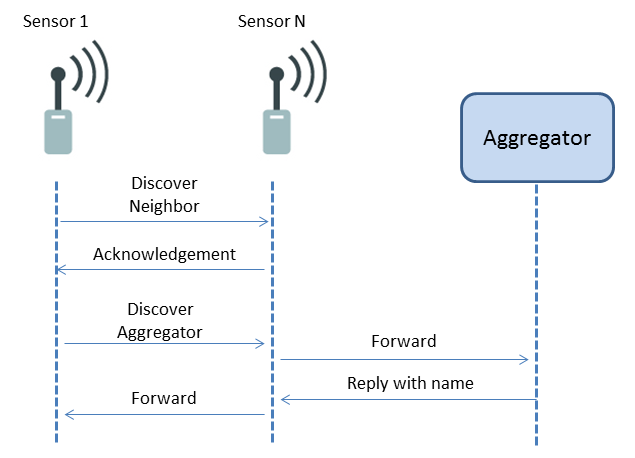
\includegraphics[width=\columnwidth]{figure/device_discovery.png}
\caption{\label{fig:device_dis}Device discovery for resource-constrained sensor}
\end{figure}



\subsection{IoT Service Discovery}

IoT services can be generally categorized into two classes: sensing and actuating. In today's IoT platforms, sensors are connected via a server, which requires considerable development effort such as maintaining a local name to IP mapping. In ICN-IoT, IoT service discovery and configuration becomes more efficient. Specifically, we consider two service discovery modes: $peer-to-peer$ and $master-slave$.


\vspace{1mm}\noindent{\bf Peer-to-peer Service Discovery}: In this mode, we consider the scenario in which an aggregator (referred to as the source aggregator) tries to discover a IoT service provided by another peer aggregator (referred to as destination aggregator). In NDN, the source aggregator broadcasts an interest using the well-known name $/area/servicename/certificate$, which will eventually reach the destination aggregator. In MF, this is handled by multicast (discussed in Section~\ref{sec:intro_mf}) instead of flooding the entire local network. All sensors that provide relevant services can join the multicast group that is identified by a $Group-GUID$. After establishing the multicast group, the source aggregator sends a request containing the service name and certificate to the multicast group.The target aggregator that hosting this service checks the certificate and registers the source Aggregator if there is a matched service. It replies with a acknowledgement containing its certificate to the source aggregator. The message flow is shown as Figure~\ref{fig:ser_dis}
\begin{figure}
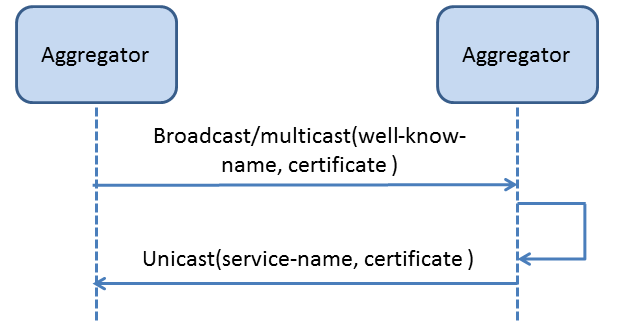
\includegraphics[width=\columnwidth]{figure/service_discovery.png}
\caption{\label{fig:ser_dis}Peer-to-peer service discovery}
\end{figure}
In an example of NDN smart home, a thermostat expresses a request to discover a AC service using well-known name $/home/ac/certificate$ via broadcast channel. In MF case, a multicast group GUID $1234$ can be assigned to all home appliance IoT service. The thermostat sends request containing the service name and certificate to $1234$. In both cases, the AC that hosting this services replies with acknowledgement if all condition match.

\vspace{1mm}\noindent{\bf Master-slave Service Discovery}:In some IoT applications, there are more than one sensing service or actuating service connecting to one control service. A source aggregator hosting control service expresses a request with service name and its certificate to discover a service from all the available aggregators. The target aggregators verify the certificate and register the source   aggregator if there is a matched service.If two condition are satisfied, they answer with acknowledgement containing their certificates.

In the AC control NDN example shown in Figure~\ref{•}, the number of AC service provider increases to three, which can be named as $/office/ac/1$, $/office/ac/2$ and $/office/ac/3$ . The thermostat expresses a partial name $/office/ac/certificate$ via a broadcast channel periodically. In the MF case, a multicast group GUID $1234$ can be assigned to identify AC service. The thermostat sends request with service name and certificate to $1234$. The target ACs reply with their certificate if the request meets all criteria.

\subsection{Secure Device Discovery, Naming Service and Service Discovery}
Security guarantee is always treated an essential function for the IoT middleware. Generally speaking, the security objective is to assure that the device that connects to the network should be authenticated, the provided services are authenticated and the data generated (through sensing or actuating) by both devices and services can be authenticated and kept privacy (if needed). To be specific, we consider the approach to secure device discovery, naming service and service discovery, because other services, such as pub/sub management and context processing \& storage, can be properly secured according to application-specific demands.
 
Recall that our goal is to assure that either device or service itself is authenticated, which attempts to prevent sybil (or spoofing) attack \cite{sybil} and the assigned name is closely binding to the device (or service). In what follows, let us consider how to secure device discovery and name assignment. Suppose that the device (i.e., sensor) can be either programmable so that before deployment the owner can preload some identity information (such as secure ID, a pair of public/private key and a certificate) , or has some manufacture ID and a pair of public/private key (which is certified by the manufacturer). That is, the device is associated with information including device identity, public/private keys ($PK_{device}, SK_{device}$) and a certificate either from the owner or the manufacturer which certifies the device identity and public/private keys. For the ICN-IoT middleware based on NDN architecture, when discovering a device, the aggregator will first verify the device identity (e.g., the device can generate a signature with the private key $SK_{device}$ and present the signature and the certificate to the aggregator so that the aggregator can verify it), and then assign a name to the device as follows: the aggregator will issues a request to LSG together with its device identity and $PK_{device}$, so that LSG can assign an ICN name and generate a certificate (certifying the binding of ICN name, $PK_{device}$). To this end, the ICN name and the certificate will be sent back to the aggregator and will be stored locally if the device is resource-restricted. Otherwise, the ICN name and the certificate will be passed to the device. For the MF-IoT, assigning a network name (GUID) for a device is rather straightforward: after verifying the device identity, the Aggregator
%generates a pair of public/private key ($PK_{mf}, SK_{mf}$), and
inserts the public key $PK_{device}$ and device information to the upper layer component to verify if there is a conflict in the corresponding scope. Specifically, LSG is in charge of local scope and IoT server guarantees the global uniqueness. Finally, the unique public key is used a GUID for the new device. Analogously, service discovery can be secured in a similar way.
 
Note that the above discussion assumes that there exists public key infrastructure (a centralized and hierarchical system) , which greatly simplify the system trust model. In some ad hoc network this assumption may not hold and some other trust mechanisms may need to be employed, such as PGP. Moreover, in order to comply with the capability of resourced-restricted devices, light-weight cryptographic primitive (such as symmetric cryptography) may be used instead of public key cryptography.

%\subsection{Secured Device Naming Service}
%A key step towards realizing a unified IoT platform is the ability to assign names that are unique within the scope and lifetime of each device, data items generated by these devices, or a group of devices towards a common objective. Naming service is usually triggered by device discovery. For NDN architecture, automatic naming scheme is following the hierarchical manor with minimum assumption -- device is always named after its attached point's name, and every physical component in our ICN-IoT middleware should have at least one name. Figure~\ref{} illustrates how a new device can be named using ICN-IoT middleware on top of NDN architecture. A sensor is being discovered by a nearby Aggregator. This Aggregator generate a key pair issues a request to the LSG with its manufacture ID and public key. On receiving of the request, the LSG generates a certificate and an ICN name for the new sensor, then send back to the Aggregator. Last, the Aggregator forward the information to the sensor or store it if the sensor has limited resource. In MF, generating a GUID for a new sensor is rather straightforward: the nearby Aggregator generates a key pair for the sensor, and inserts the public key and device information to the upper layer component to verify if there is a conflict in the corresponding scope. Specifically, LSG is in charge of local scope and IoT server guarantees the global uniqueness.Finally, the unique public key is used a GUID for the new device.

\subsection{Publish/Subscribe Management}
Data Publish/Subscribe (Pub/Sub) is an important function for ICN-IoT, response for resource sharing and management. In conventional IP network, most of the IoT platforms provide a centralized server to aggregate all IoT service and data. While resource is being published as service,  centralized architecture ensures the availability, but it poorly supports scalability and high bandwidth consumption due to high volume of control and data exchange. Thus, we consider a decentralized pub/sub model in ICN-IoT middleware. Specifically, we will discuss rendezvous mode and a data-control separated mode.

\vspace{1mm}\noindent{\bf Rendezvous Mode}:Rendezvous mode is classical pub/sub scheme in which data and request meet at a intermediate node. NDN is a Pull-based architecture, where the Pub/Sub is not naturally supported , but COPSS~\cite{chen2011copss} proposes a solution for such requirement. It integrates a push based multicast feature with the pull based NDN architecture at the network layer by introducing Rendezvous Node(RN). RN is logical entity that reside in NDN node. The publisher first forwards a Content Descriptor (CD) as a snapshot to the RN. RN maintains a subscription table, and receives the Subscription message from subscriber. The data publisher just sends the content using Publish packet by looking up FIB instead of PIT. If the same content root is required by multiple subscribers. RN will deliver one copy  of content downstream, hence reduced bandwidth consumption.

\vspace{1mm}\noindent{\bf Data-control separated Mode}:Compared with Rendezvous mode in which data plane and control plane both reside on the same ICN network layer, we consider a architecture that centralized server takes over the control message while data is handled by ICN network layer. Following the naming process mentioned above, the LSG has the ICN name for the local resource which is available for publishing on IoT server. IoT server maintains the subscription membership, and receives subscription request from subscriber. Due to the precise number and identify of the resource provider is unknown for the subscriber in a dynamic scenario, IoT server also takes responsibility of grouping and assigning group name for the resource. The generic message flow for publish/subscribe function is shown in Figure~\ref{fig:pubsub}, and we will introduce the detail in each individual architecture.
In NDN, the grouping resource is intuitive : all resource have the same schematic prefix will be grouped together, and the prefix can be used to identify the service. The traditional NDN dose not support using a a common partial name to retrieve multiple resource, but M. Amadeo et al. ~\cite{amadeo2014multi} provide solution that resolves this issue by introducing long-life multi-source Interest in PIT.
MF takes advantage of  $Group-GUID$ to identify a service formed by multiple resource. This $Group-GUID$ will be distributed to the subscriber as well as the publisher. In an example of NDN,  it uses the common prefix$/home/monitoring/$ to identify a group of resource that provides multiple monitoring service such as $/home/monitoring/temperature$ and $/home/monitoring/light$. The subscriber retrieves the prefix from IoT server, and sends Interest toward the resource. In a MF example, $GUID-x$ identifies the "home monitoring" service that combines with "light status" and "temperature". The resource producers, i.e. the host of "temperature" and the host of "light status" are notified that their service belong to $GUID-x$, then listen on $GUID-x$. The subscriber sends request toward  $GUID-x$, and request will be multicasted to the producers at the last common node. On receiving the request, the resource producer unicasts the data to the subscriber. Moreover, if multiple resource consumers subscribe to the same resource,
the idea of $Group-GUID$ can be reused here to group the consumers to further save bandwidth using multicast.
\begin{figure}
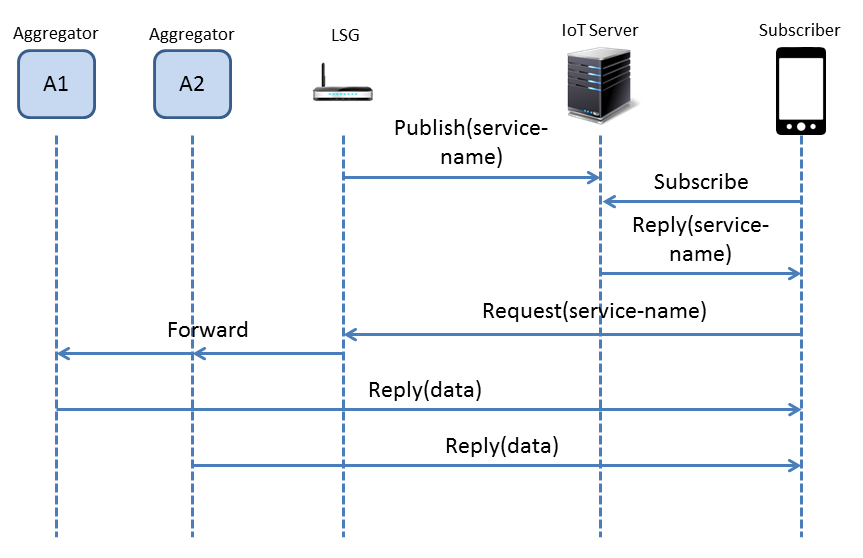
\includegraphics[width=\columnwidth]{figure/pub_sub.png}
\caption{\label{fig:pubsub}Publish/subscriber management message flow}
\end{figure}
